\documentclass[10pt,letterpaper,spanish,twoside]{report}

\usepackage{practica}
\usepackage{graphicx}
\usepackage{float}
\DeclareGraphicsExtensions{.bmp,.png,.pdf,.jpg}
\newcommand{\docdate}{
  \vspace{2em}
   \begin{flushright}
     Ciudad de México. \datedayname~\today.
   \end{flushright}
  \vspace{2em}
}

\begin{document}
\docdate

\begin{center}
 \textsc{\asignatura}\vspace{.2em}
\end{center}

\textsc{Manual del profesor}\vspace{.2em}

\textsc{Práctica 3. aplicación de filtros digitales tipo butterworth rechaza banda a señales biomédicas reales}

\textsc{Objetivo:} Aplicar los conocimientos sobre el diseño de filtros Butterwoth digitales rechaza banda para procesamiento de señales biomédicas reales.

\textsc{Actividades}
\begin{enumerate}
 \item Descargar el archivo 'PCG$\_$60.npz' disponible en 
 \item Se recomienda reproducir el audio, para identificar que la señal se encuentra contaminada, se puede consultar en el script 'Butterworth$\_$practica3'. 
 \\ Si se desea hacer alguna modificación en la señal de PCG se puede consultar el script 'señales utilizadas'.
 \\En la figura~\ref{contexto:PCG} se muestra la señal de PCG, es porsible observar un ruido alrededor de los 17 segundos que indica que posiblemente fue producida por un artefacto de movimiento.
 \begin{figure}[H]
 	\centering
 	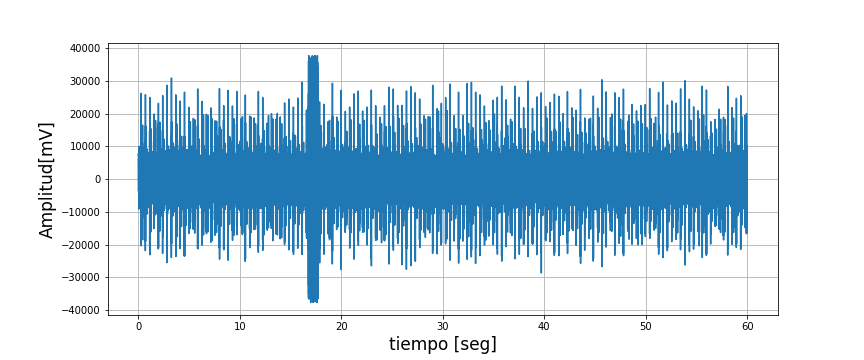
\includegraphics[scale=0.5]{PCG.PNG}
 	\caption{Señal de PCG}
	\label{contexto:PCG}
 \end{figure}
 \item Obtener la FFT de la señal de manera digital, esto es posible realizarlo con la función fou, en la figura~\ref{contexto:FFT_c} es posible observar que la interferencia se encuentra en los 60 Hz 
 \begin{figure}[H]
 	\centering
 	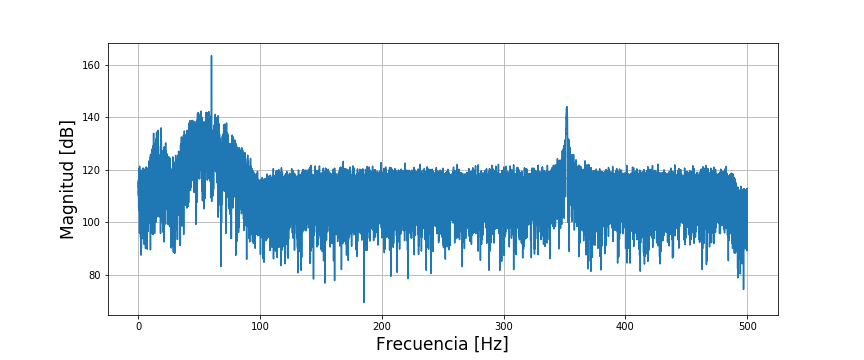
\includegraphics[scale=0.5]{FFT_c.PNG}
 	\caption{FFT de señal de PCG}
 	\label{contexto:FFT_c}
 \end{figure}
 \item Para el diseño del filtro rechaza banda orden 2 se recomienda utilizar frecuencias de corte de 58 y 62 Hz para eliminar el ruido de línea (la frecuencia de corte debe estar normalizada). En la figura~\ref{contexto:RF_RB2} se muestra la respuesta en frecuencia del filtro.
 \begin{figure}[H]
 	\centering
 	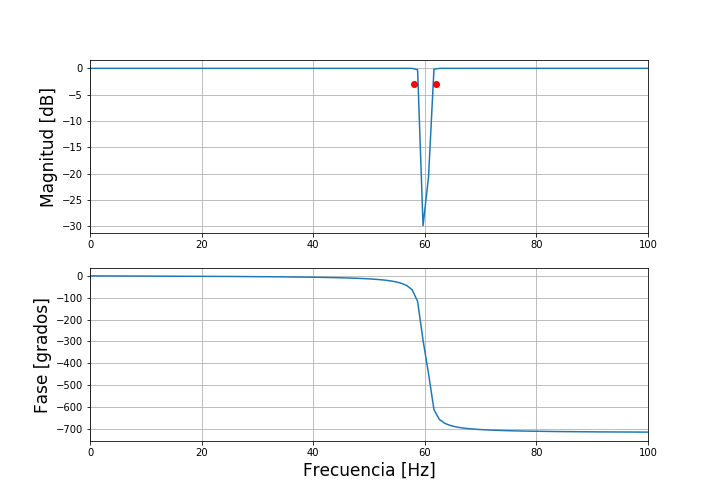
\includegraphics[scale=0.5]{RF_RB2}
 	\caption{Respuesta en frecuencia del filtro rechaza banda orden 2}
 	\label{contexto:RF_RB2}
 \end{figure}
 \begin{enumerate}
 	\item Se puede observar en puntos rojos que las frecuencias de corte se encuentran en 58 y 62 Hz.
 	\item En la gráfica de fase se puede observar que el desfase es lineal.
 \end{enumerate}
 \item Se procede a filtrar la señal en fase cero, lo que quiere decir que la señal será filtrada dos veces, esto para evitar desfase de la señal. En la figura~\ref{contexto:FFT_RB2} se observa la FFT de la señal filtrada en fase cero. 
 \begin{figure}[H]
	\centering
	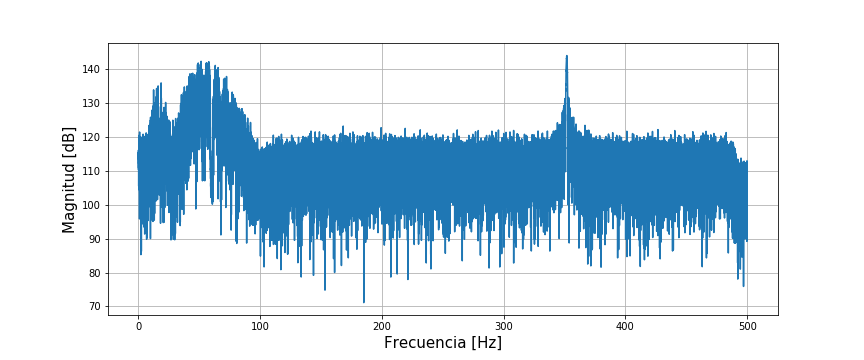
\includegraphics[scale=0.45]{FFT_RB2}
	\caption{FFT de la señal filtrada con filtro de orden 2}
	\label{contexto:FFT_RB2}
 \end{figure} 
 \begin{enumerate}
 	\item Comparando la FFT de la figura~\ref{contexto:FFT_c} y \ref{contexto:FFT_RB2} es posible observar que el ruido de 60 Hz fue eliminado correctamente 
 	\item Para valorar la funcionalidad del filtro, es necesario reproducir la señal de fonocardiograma para detectar si la interferencia fue eliminada correctamente
 \end{enumerate}  
 \item Para el diseño del filtro rechaza banda de orden 4 se modificaran las frecuencias de corte y se sugiere utilizar 59 y 61 Hz. En la figura~\ref{contexto:RF_RB4} se muestra la respuesta en frecuencia del filtro.
 \begin{figure}[H]
 	\centering
 	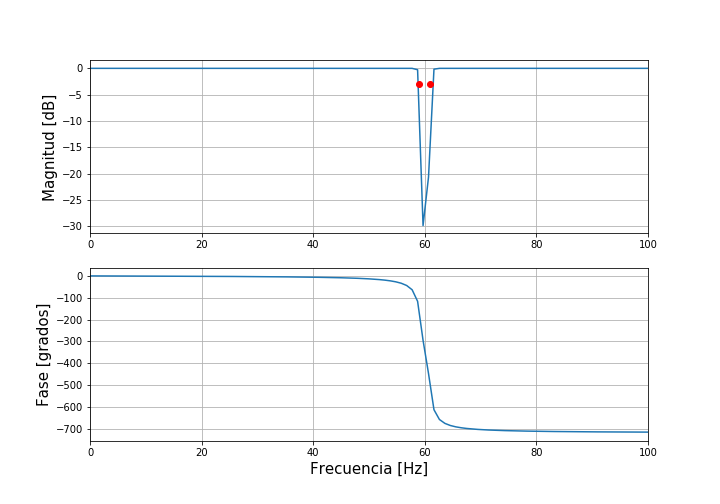
\includegraphics[scale=0.45]{RF_RB4}
 	\caption{Respuesta en frecuencia del filtro orden 4}
 	\label{contexto:RF_RB4}
 \end{figure}
 \begin{enumerate}
 	\item Se puede observar que las frecuencias de corte se encuentran aprox en 59 y 61 Hz, así también, es posible notar que la fase tiene un comportamiento lineal
 \end{enumerate}
 \item Se filtrará la señal en fase cero como en el caso del filtro anterior. En la figura~\ref{contexto:FFT_RB4} se observa la FFT de la señal filtrada con filtro de orden 4.
 \begin{figure}[H]
 	\centering 
 	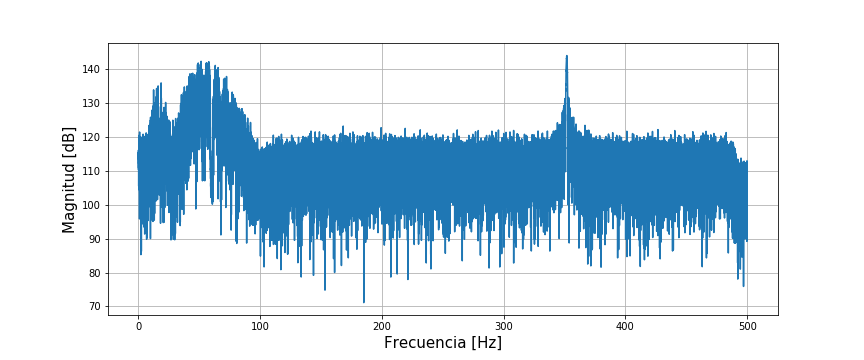
\includegraphics[scale=0.5]{FFT_RB4}
 	\caption{FFT de la señal filtrada con filtro de orden 4}
 	\label{contexto:FFT_RB4}
 \end{figure}
 \begin{enumerate}
 	\item Comparando la FFT de la figura~\ref{contexto:FFT_c} y \ref{contexto:FFT_RB4} se puede observar que el ruido de línea fue eliminado correctamente
 	\item Para valorar el funcionamiento del filtro es necesario reproducir la señal de PCG.
 \end{enumerate}
\end{enumerate}


%\textsc{Nota}
%\vspace{2em}
\vfill
\begin{flushright}
\textsc{Elaboró:\\
Ma. del Rosario Aguilar Cruz\\
Enrique Mena Camilo}
\end{flushright}

\end{document}